\pagenumbering{gobble}
\vspace{-1cm}
\begin{minipage}[t][5cm][t]{1.13\textwidth}
\maketitle
\end{minipage}

\begin{tikzpicture}[remember picture,overlay,inner sep=0pt,outer sep=0pt]
	\node at (9.5cm,-10cm) {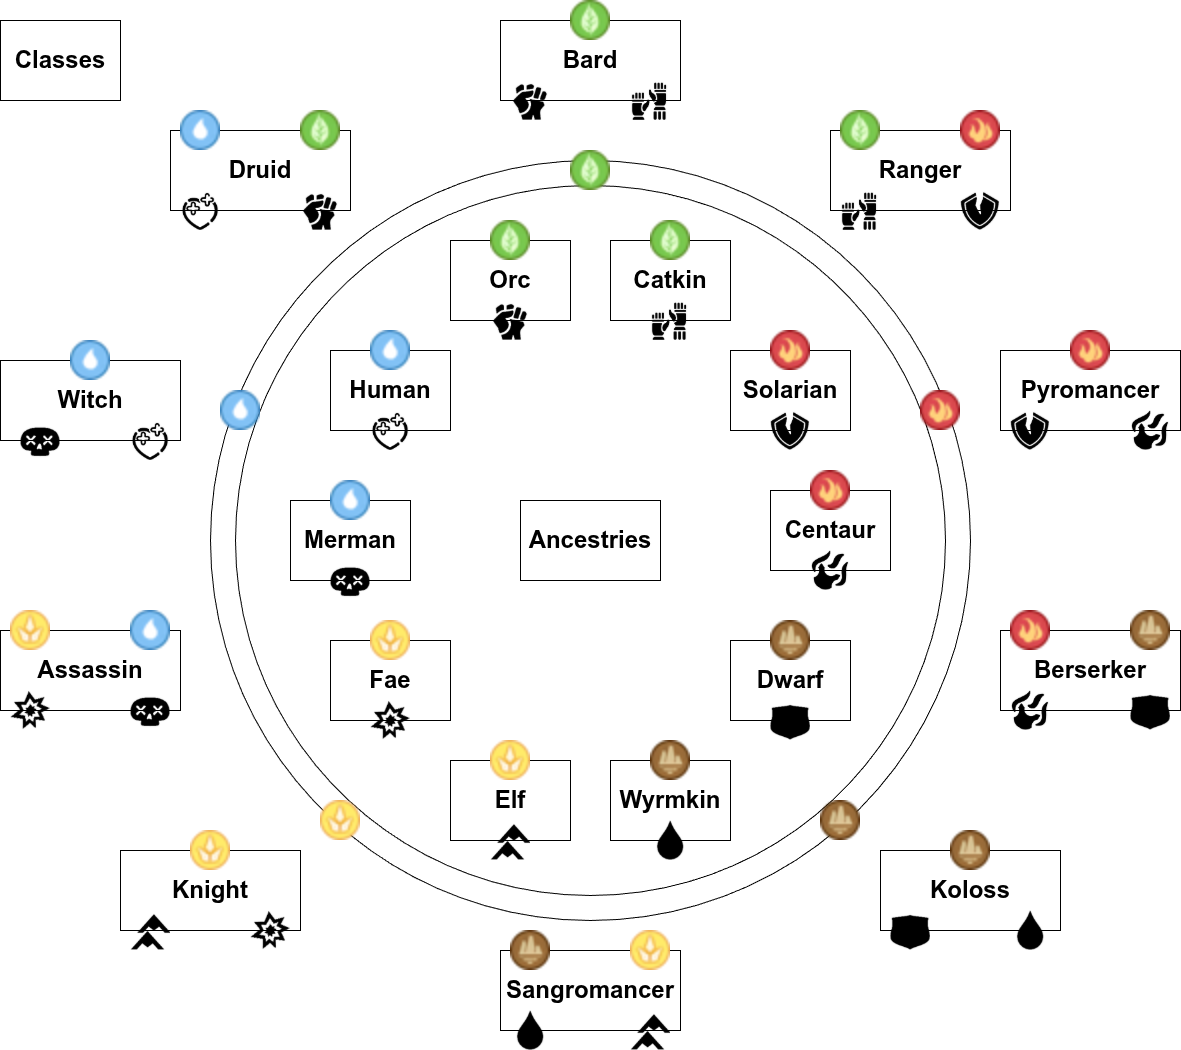
\includegraphics[width=0.8\paperwidth]{../GuidePics/Circle_Mechanics.drawio.png}};
\end{tikzpicture}

\vspace{18cm}
Players: 3-5\\
Game Time: 2-3h

\newpage

\pagenumbering{arabic}
%\section{Foreword} This one wont have a section formatting, but still needs to be there

%All primers need to be in here. This includes: Multiclassing, deckbuilding, the modifier deck, Co-op, species?, roguelike?, Wheelgame?,
\begin{minipage}[t][15.5cm][t]{0.5\textwidth}
	\begin{minipage}[t][14cm][t]{0.9\textwidth}

		
		
		\textbf{Rule 0}: The game is about having fun. If you and your playgroup decide that some change to the rules would increase your fun, experiment with it!
		
			\fbox{\parbox[4cm]{\textwidth}{Large space for lore and pictures}}

	\end{minipage}
\end{minipage}
\begin{minipage}[t][12cm][t]{0.5\textwidth}
	\setlength{\cftbeforetoctitleskip}{-0.5em}
	\setlength{\cftbeforesecskip}{0em}
	\tableofcontents
	

\end{minipage}
